\documentclass{amsart}
\usepackage[utf8]{inputenc}
\usepackage{enumerate}
\usepackage{graphicx}

\theoremstyle{definition}
\newtheorem{problem}{Příklad}



\begin{document}

\section*{Cvičení z logiky: 2. sada příkladů}

\bigskip\bigskip\bigskip

\subsection*{Témata:} 

Teorie. Normální formy, CNF a DNF, SAT a 3-SAT. 2-SAT a implikační graf. Horn-SAT a jednotková propagace. Kódování problémů do SAT.


\bigskip

\hrule

\bigskip\begin{problem}
Mějme teorii $T=\{\neg q \to (\neg p \vee q),\ \neg p \to q,\ r \to q\}$ v jazyce $\{p, q, r, s\}$. Které z následujících výroků jsou pravdivé, lživé, nezávislé, splnitelné, ekvivalentní v teorii $T$?
\begin{enumerate}[(a)]
\item $p$, $q$, $r$, $s$, $\neg p$, $\neg s$
\item $p \vee q$,\ $p \vee r$,\ $p \vee s$,\ $q \vee s$
\item $p \wedge q$,\ $q \wedge s$,\ $p \to q$,\ $s \to q$
\end{enumerate}
\end{problem}

\hrule

\bigskip\begin{problem} Pro danou formuli $\varphi$ v CNF nebo DNF, A) určete počet modelů a B) popište množinu všech modelů.
\begin{enumerate}[a)]
\item $(p_1 \wedge  \neg p_2 \wedge  p_3 \wedge  \neg p_4 )\vee(p_2 \wedge  p_3 \wedge  \neg p_4 )\vee(\neg p_3)\vee(p_2 \wedge  p_4)\vee(p_1 \wedge  p_3 \wedge  p_5 )\vee(p_3 \wedge  \neg p_4 \wedge  p_2 )$
\item $(p_1 \vee \neg p_2 \vee p_3 \vee \neg p_4 )\wedge(p_2 \vee p_3 \vee \neg p_4 )\wedge(\neg p_3)\wedge(p_2 \vee p_4)\wedge(p_1 \vee p_3 \vee p_5 )\wedge(p_3 \vee \neg p_4 \vee p_2 )$
\end{enumerate}
\end{problem}






\bigskip\begin{problem} Převeďte následující výroky do CNF a DNF A) tabulkou (určením modelů), B) ekvivalentními
úpravami.
\begin{enumerate}[a)]
    \item $(\neg p \vee q)\to (\neg q \wedge r)$,
    \item $(\neg p \to (\neg q \to r))\to p$,
    \item $((p\to \neg q) \to \neg r) \to \neg p$.

\end{enumerate}
\end{problem}




\bigskip\begin{problem} Pro danou formuli $\varphi$ v CNF najděte a 3-CNF formuli $\varphi'$ takovou, že $\varphi'$ je splnitelná, právě když $\varphi$ je splnitelná. Popište efektivní algoritmus konstrukce $\varphi'$ je-li dána $\varphi$ (tj. redukci z problému SAT do problému 3-SAT).
\end{problem}


\bigskip\begin{problem} Najděte (co nejkratší) CNF a DNF reprezentace Booleovské funkce $\mathrm{maj}: {^3}2\to 2$, která vrací převládající hodnotu mezi 3 vstupy.
\end{problem}


\bigskip\begin{problem} Uměli byste nalézt CNF a DNF reprezentace $n$-ární parity, tj. Booleovské funkce $\mathrm{par}: {^n}2\to 2$ definované pomocí $\mathrm{par}(x_1,\dots,x_n)=(x_1+\dots+x_n)\bmod 2$,
která vrací XOR všech vstupních hodnot? Zkuste to pro malé hodnoty $n$.
\end{problem}


\bigskip\begin{problem} Buď $\mathbb P$ spočetně nekonečná množina prvovýroků. Ukažte, že již neplatí, že každou $K\subseteq {^\mathbb P}2$ lze namodelovat výrokem v CNF i výrokem v DNF. Najděte množinu modelů $K$, kterou nelze namodelovat $K$ ani v CNF, ani v DNF.
\end{problem}







% \bigskip\begin{problem}
% Označme $\mathrm{maj}_n: {^3}({^n}2)\to {^n}2$ $n$-ární majoritu po složkách, tj. například
% $$
% \mathrm{maj}_4((0, 1, 0, 1),(1, 1, 0, 0),(1, 1, 0, 0)) = (1, 1, 0, 0).
% $$
% Množina $K\subseteq {^n}2$ je \emph{mediánová}, pokud je uzavřená na $\mathrm{maj}_n$.
% \begin{enumerate}[a)]
%     \item Ukažte, že pro každý 2-CNF výrok $\varphi$ je $M(\varphi)$ mediánová.
%     \item* Ukažte, že pro každou mediánovou množinu $K\subseteq {^n}2$ existuje 2-CNF výrok $\varphi$ nad  $n$ proměnnými takový, že $M(\varphi) = K$.
%     %\item** Jak je to s$n$-ární paritou po složkách?
% \end{enumerate}
% \end{problem}


\hrule


\bigskip\begin{problem} Sestrojte implikační graf daného 2-CNF výroku. Je splnitelný? Pokud ano, najděte nějaké řešení.
\begin{enumerate}[a)]
\item $(p_1\vee \neg p_2)\wedge (p_2\vee p_3)\wedge (\neg p_3\vee \neg p_1)\wedge (\neg p_3\vee \neg p_4)\wedge (p_4\vee p_5)\wedge (\neg p_5\vee \neg p_1)$,
\item $(p_1\vee \neg p_2)\wedge (p_2\vee p_3)\wedge (\neg p_3\vee p_1)\wedge (\neg p_3\vee \neg p_4)\wedge (p_4\vee p_5)\wedge (\neg p_5\vee p_1)$,
\item $(p_0 \vee  p_2) \wedge  (p_0 \vee  \neg p_3) \wedge  (p_1 \vee  \neg p_3) 
\wedge  (p_1 \vee  \neg p_4) \wedge  (p_2 \vee  \neg p_4) 
\wedge  (p_0 \vee  \neg p_5)
\wedge 
(p_1 \vee  \neg p_5) \wedge  (p_2 \vee  \neg p_5) \wedge  (\neg p_1 \vee  \neg p_6) \wedge  (p_4 \vee  p_6) \wedge  (p_5 \vee  p_6) \wedge  p_1\wedge \neg p_7$.
\end{enumerate}
\end{problem}

\begin{problem}
Pomocí jednotkové propagace zjistěte, zda je následující Hornův výrok splnitelný. Pokud ano, najděte nějaké splňující ohodnocení.
\begin{align*}
&(\neg p_1 \vee \neg p_3 \vee p_2)\wedge(\neg p_1 \vee p_2)\wedge p_1 \wedge (\neg p_1 \vee \neg p_2 \vee p_3)\wedge \\
&(\neg p_2 \vee \neg p_4 \vee p_1)\wedge(\neg p_4 \vee \neg p_3 \vee \neg p_2)\wedge(p_4\vee \neg p_5 \vee\neg p_6)
\end{align*}
\end{problem}


\hrule


\begin{problem}
Lze šachovnici $4\times 4$ bez dvou protilehlých rohů perfektně pokrýt kostkami domina? Zakódujte tento problém do SAT. Zobecněte na všechna sudá~$n$.
\end{problem}


\begin{problem}
Lze obarvit čísla od 1 do $n$ dvěma barvami tak, že neexistuje monochromatické řešení rovnice
$a+b=c$ s $1\leq a<b<c\leq n$? Sestrojte výrokovou formuli $\varphi_n$ v CNF která je splnitelná, právě když to lze. Zkuste nejprve $n=8$.

Zkuste si doma: Napište skript generující $\varphi_n$ v DIMACS CNF formátu. Použijte SAT solver k nalezení nejmenšího $n$ pro které takové obarvení neexistuje (tj. každé 2-obarvení obsahuje monochromatickou trojici $a<b<c$ takovou, že $a+b=c$).
\end{problem}



\begin{problem}
Zakódujte problém setřídění trojice celých čísel do SAT.
\end{problem}



\begin{problem}
Slavná Věta o čtyřech barvách říká, že následující mapu lze obarvit 4 barvami tak, že žádné dva sousedící regiony nemají stejnou barvu. Najděte takové obarvení (pomocí SAT solveru).
\begin{center}
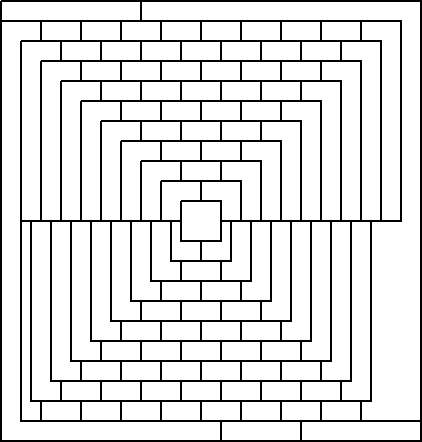
\includegraphics[width=0.8\textwidth]{files/map.png}
\end{center}
\end{problem}

\end{document}.